\documentclass[a4paper,oneside]{article}

  \usepackage{graphicx}
  \usepackage{subcaption}
  \usepackage{xcolor}
  \usepackage{hyperref}
  \usepackage[cm]{fullpage}
  \usepackage{booktabs}
  \usepackage{lmodern} 
  \usepackage[T1]{fontenc}
  \usepackage{amsmath}

\begin{document}
  \section*{The hypothetical adaptive value of the generalized growth arrest and the constraints for a successful sex event}
    Molecular, biophysical and chemical data discussed above unequivocally show that \textit{P.~multistriata}, during events of mating and gametogenesis, blocks growth and mitosis for a few days --- three in the experiment discussed here, and up to six in the one discussed by Scalco et al. (2014).
    Also, cell number decreases, very likely for enhanced mortality due to the gametogenesis.

    To analyze the impact of such behaviour on population dynamics, we developed a simple process-based model of growth dynamics during the sexual reproduction event, where net growth is the balance between size-dependent cell growth and death.
    \textbf{The model is conceptually zero-dimensional, and the initial conditions consider the minimal cell concentration recorded by Scalco et al. (2014) as gametogenesis trigger.
    Cell numbers and available Nitrogen are expressed as abundance and concentration, respectively.}
    
    The simulation starts with a cell population ($P$) that enters the sexual reproduction phase after reaching a threshold value of a few thousand cells per ml (see Scalco et al., 2014).
    During this phase of variable length, the population stop growing and experience a prolonged burst of extra mortality.
    Within the same span, a $P$ fraction will undergo gametogenesis and generate an offspring population ($F_{1}$) that will start to grow the moment ($t_{F_{1}I}$) it appears.
    After $t_{AE}$ days, the growth arrest will end and $P$ will resumes its growth alongside $F_{1}$.

    During the entire course of the simulation (set to ten days) cell growth is modulated by competition over Nitrogen and by cell size via an allometric relationship (see D'Alelio et al., 2010).
    A fundamental assumption, discussed later in the text, is that parental and daughters cells share a common, exclusive space, so that only $P$ and $F_{1}$ compete for N made available in such space.
    This assumption is translated in the model as a decrease in growth rate as the total population ($F_{1} + P$) converges toward the carrying capacity, set as the total nitrogen content of initial parental cells.
    
    To understand better how event timing and response amplitudes impact over $F_1$ recruitment success, we compared simulation outputs across selected parameters range.
    Our selected parameters are the $P$ fraction that will generate $F_{1}$ ($\alpha$), gametogenesis-induced extra mortality of parental cells ($d$), duration of the growth arrest ($t_{AE}$), and growth rates ratio among parental and initial cells ($r_{P}:r_{F_{1}}$)
    We deployed an interactive version of the model at the URL \url{https://arfalas.shinyapps.io/pns_toy/}, code and figures are available on \url{https://github.com/bhym/Stec} ({\color{red} currently private})
%
  \section*{Model description}
    Parental ($P$) and offspring ($F1$) dynamics are defined as ODE:\@
    %
    \begin{align}
      \frac{dP}{dt}     &= \kappa \beta_{P} P - \delta P \\
      \frac{dF_{1}}{dt} &= \kappa \beta_{F_{1}} F_{1}
    \end{align}
    %
    where $\kappa$ is the competition for N, defined as
    \[
      1 - \frac{{[N]}_{t}}{1.2{[N]}_{t=0}}
    \]
    with 
    \[
      N_{t} = {[P]}_{t} {[N]}_{P} + {[F_{1}]}_{t} {[N]}_{F_{1}}
    \]

    $\beta_{P}$ and $\beta_{F_{1}}$ are defined as
    \[
      \beta_{P} =
        \begin{cases}
          0                    & \mbox{if } t <    t_{AE} \\
          \lambda_{P}(t) r_{P} & \mbox{if } t \geq t_{AE}
        \end{cases}
      \qquad;\qquad
      \beta_{F_{1}} = 
        \begin{cases}
          0                            & \mbox{if } t <    t_{F_{1}I} \\
          \lambda_{F_{1}}(t) r_{F_{1}} & \mbox{if } t \geq t_{F_{1}I}
        \end{cases}
    \]
    with $\lambda_i(t)$ representing allometric scaling on length ($L$), defined as
    \[
      \lambda_{i}(t) = 0.25 + 0.04 L_{i}(t) - 0.0005 L_{i}{(t)}^{2}
    \]
    Length dynamics are based on cell's age ($a$) and are defined by the rule
    \[
      L_{i}(t) = L_{0,i} - 0.1 a(t) \hspace{8mm}\text{with $i$ either $P$ or $F_{1}$}
    \]
    Age is counted from the appearance of the population, and does not increase during GA.\@

    Finally, $\delta$ is an extra mortality term defined as
    \[
      \begin{cases}
        d & \mbox{if } t < t_{AE} \\
        0 & \mbox{if } t > t_{AE}
      \end{cases}
    \]
    The parameters values and ranges are reported in \textbf{Table~\ref{tbl1}}.
    %
    \begin{table}
      \centering
      {%
        \begin{tabular}{@{}llccr@{}}
          \toprule
          \textbf{Variable}&\textbf{Meaning} & \textbf{Units} & \textbf{Value} & \textbf{Reference}\\
          \midrule
          ${P}_{0}$       & initial concentration of $P$ cells         & cells/ml          & 4E3         & Experiment detailed in the paper\\
          $\alpha$        & fraction of $P$ that will generate $F_{1}$ & ---               & [0.01, 0.2] & Explored via simulations\\
          $r_{P}$         & net growth rate of $P$                     & $\text{day}^{-1}$ & [1, 3]      & Explored via simulations\\ 
          $r_{F_{1}}$     & net growth rate of $F_{1}$                 & $\text{day}^{-1}$ & 1           & ---\\
          $t_{AE}$        & end day of the growth arrest               & day               & [2,6]       & Explored via simulations\\
          $t_{F_{1}I}$    & day of appearence of the offspring         & day               & 3           & Experiment detailed in the paper\\
          $L_{0,P}$       & starting length for $P$ cells              & $\mu$m            & 40          & Experiment detailed in the paper\\
          $L_{0,{F_{1}}}$ & starting length for $F_{1}$ cells          & $\mu$m            & 80          & Experiment detailed in the paper\\
          $d$             & gametogenesis-induced extra mortality      & day               & [0.1, 0.9]  & Explored via simulations\\
          \bottomrule
        \end{tabular}
       }
      \caption{Values and ranges for model parameters}\label{tbl1}
    \end{table}
%
  \section*{Results}
    \textbf{Fig.~\ref{fdyn}} shows the relative variation of allometric growth (panel a), the size reduction of $P$ and $F_{1}$ during the simulations (panel b) and variation of $P$ and $F_{1}$ densities for two different sets' of parameter values (panels c and d) \textbf{reported in the legend}.
    We simulated a wide set of scenarios corresponding to the chosen ranges of variation of the different parameters reported in \textbf{Table~\ref{tbl1}} focusing, as output variable, on the recruitment success of the offsprings quantified as the ratio between $F_{1}$ and $P$, after ten days from the start of mating.
    \textbf{Fig.~\ref{swep}} shows the logarithm of the ratio in relation to different values of the parameters or their combination.
    %
    \begin{figure}[p]
      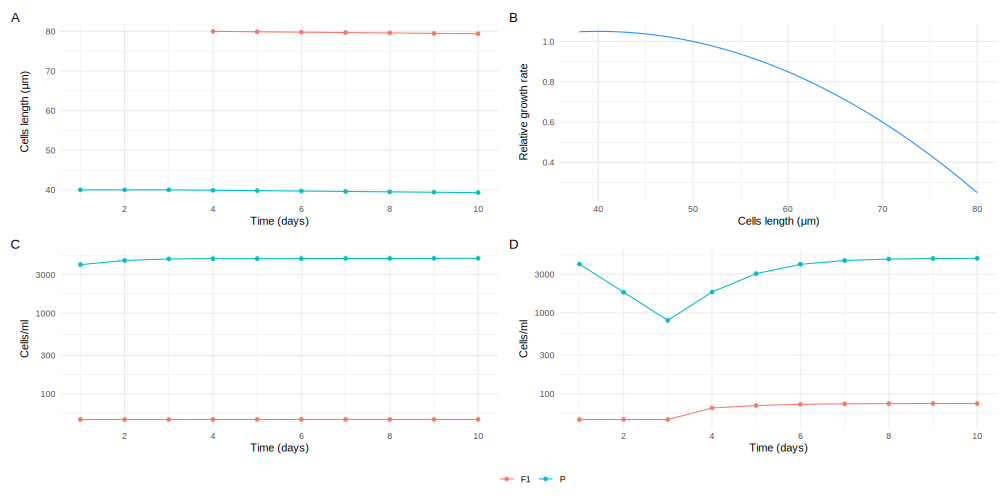
\includegraphics[width=\linewidth]{imgs/Figpan.pdf}
      \caption{\textbf{Simulated size dependent growth and impact on the population dynamics} ---
      \textit{(a)} dependence of specific growth rate on cell length;
      \textit{(b)} Size reduction for the two sub-populations;
      examples of simulation outputs whith $r_{p} = 1.82$ \textit{(c)} and $r_{p} = 1$ \textit{(d)}.
      In \textit{(c)} and \textit{(d)}: $\alpha=0.012, d = 0.8$, all the other parameters as per \textbf{Tab.~\ref{tbl1}}.}\label{fdyn}
    \end{figure}
    %
    \begin{figure}[p]
      \centering
      \begin{subfigure}{\textwidth}
        \includegraphics[width=\linewidth]{imgs/a.pdf}
      \end{subfigure}

      \begin{subfigure}{\textwidth}
        \includegraphics[width=\linewidth]{imgs/b.pdf}
      \end{subfigure}
      \caption{\textbf{Contour plots of ranges of recruitment success after 10 days of simulation for paired values of parameters (axes labels).}
      Recruitment success is expressed as $\log(\frac{F_1}{P})$; $\alpha$ is the fraction of $P$ cells that will generate $F_{1}$.
      Different subplots represent different durations of growth arrest ($t_{AE}$ model parameter).
      }\label{swep}
    \end{figure}
    %
    \begin{table}[p]
      \centering
      {%
        \begin{subtable}{12cm}\centering\scriptsize
          {
\begin{tabular}{lrrrrrrrrr}
\toprule{}
  & 0.01 & 0.03 & 0.05 & 0.08 & 0.1 & 0.12 & 0.15 & 0.17 & 0.2\\
\midrule{}
3 & -1.88 & -1.40 & -1.16 & -0.94 & -0.83 & -0.74 & -0.63 & -0.56 & -0.47\\
2.7 & -1.88 & -1.39 & -1.16 & -0.94 & -0.83 & -0.74 & -0.62 & -0.56 & -0.47\\
2.5 & -1.88 & -1.39 & -1.16 & -0.94 & -0.83 & -0.74 & -0.62 & -0.56 & -0.47\\
2.2 & -1.87 & -1.39 & -1.15 & -0.93 & -0.82 & -0.73 & -0.62 & -0.55 & -0.46\\
2 & -1.87 & -1.38 & -1.15 & -0.93 & -0.82 & -0.73 & -0.62 & -0.55 & -0.46\\
\addlinespace
1.7 & -1.86 & -1.37 & -1.14 & -0.92 & -0.81 & -0.72 & -0.61 & -0.54 & -0.46\\
1.5 & -1.86 & -1.37 & -1.14 & -0.92 & -0.81 & -0.72 & -0.61 & -0.54 & -0.45\\
1.2 & -1.84 & -1.35 & -1.12 & -0.90 & -0.80 & -0.71 & -0.59 & -0.53 & -0.44\\
1 & -1.83 & -1.34 & -1.11 & -0.89 & -0.78 & -0.69 & -0.58 & -0.52 & -0.43\\
\bottomrule{}
\end{tabular}
}
          \caption{$\alpha, r_p:r_{f1}, \text{with } d = 0.2$}
        \end{subtable}
        \\
       \vspace{0.5cm}
        \begin{subtable}{12cm}\centering\scriptsize
          {
\begin{tabular}{lrrrrrrrrr}
\toprule
  & 0.01 & 0.03 & 0.05 & 0.08 & 0.1 & 0.12 & 0.15 & 0.17 & 0.2\\
\midrule
3 & -1.56 & -1.06 & -0.83 & -0.60 & -0.49 & -0.39 & -0.27 & -0.20 & -0.10\\
2.7 & -1.55 & -1.06 & -0.82 & -0.59 & -0.48 & -0.39 & -0.26 & -0.19 & -0.10\\
2.5 & -1.55 & -1.05 & -0.82 & -0.59 & -0.48 & -0.38 & -0.26 & -0.19 & -0.09\\
2.2 & -1.54 & -1.05 & -0.81 & -0.58 & -0.47 & -0.37 & -0.25 & -0.18 & -0.09\\
2 & -1.53 & -1.04 & -0.80 & -0.57 & -0.46 & -0.37 & -0.25 & -0.17 & -0.08\\
\addlinespace
1.7 & -1.52 & -1.03 & -0.79 & -0.56 & -0.45 & -0.35 & -0.23 & -0.16 & -0.07\\
1.5 & -1.51 & -1.01 & -0.78 & -0.55 & -0.44 & -0.34 & -0.22 & -0.15 & -0.06\\
1.2 & -1.48 & -0.99 & -0.75 & -0.52 & -0.41 & -0.32 & -0.20 & -0.13 & -0.04\\
1 & -1.46 & -0.96 & -0.72 & -0.50 & -0.39 & -0.29 & -0.18 & -0.11 & -0.02\\
\bottomrule
\end{tabular}
}
          \caption{$\alpha, r_p:r_{f1}, \text{with } d = 0.4$}
        \end{subtable}
        \\
       \vspace{0.5cm}
        \begin{subtable}{12cm}\centering\scriptsize
          {
\begin{tabular}{lrrrrrrrrr}
\toprule
  & 0.01 & 0.03 & 0.05 & 0.08 & 0.1 & 0.12 & 0.15 & 0.17 & 0.2\\
\midrule
3 & -0.37 & 0.18 & 0.44 & 0.67 & 0.77 & 0.85 & 0.93 & 0.97 & 1.02\\
2.7 & -0.31 & 0.24 & 0.50 & 0.72 & 0.82 & 0.89 & 0.97 & 1.01 & 1.05\\
2.5 & -0.27 & 0.28 & 0.54 & 0.76 & 0.85 & 0.92 & 0.99 & 1.03 & 1.07\\
2.2 & -0.18 & 0.37 & 0.61 & 0.82 & 0.90 & 0.96 & 1.03 & 1.07 & 1.11\\
2 & -0.12 & 0.43 & 0.67 & 0.86 & 0.94 & 1.00 & 1.06 & 1.09 & 1.13\\
\addlinespace
1.7 & 0.01 & 0.54 & 0.75 & 0.93 & 1.00 & 1.05 & 1.10 & 1.13 & 1.16\\
1.5 & 0.12 & 0.62 & 0.82 & 0.97 & 1.04 & 1.08 & 1.13 & 1.16 & 1.19\\
1.2 & 0.31 & 0.75 & 0.92 & 1.05 & 1.10 & 1.14 & 1.18 & 1.20 & 1.22\\
1 & 0.46 & 0.84 & 0.99 & 1.10 & 1.14 & 1.18 & 1.21 & 1.23 & 1.25\\
\bottomrule
\end{tabular}
}
          \caption{$\alpha, r_p:r_{f1}, \text{with } d = 0.6$}
        \end{subtable}
        \caption{Tabular data of $\log(\frac{F_1}{P})$ for different values of parameters showed at bottom and growth arrest duration of four days. All other parameters  as per \textbf{Tab.~\ref{tbl1}}}\label{tbl2}
      }
    \end{table}
%
  \section*{Assumptions} 
    \begin{enumerate}
      \item I assume that net growth rate is the difference between size-dependent cell growth and death
      \item I assume that $P$ suffers extra mortality during growth arrest due to gametogenesis
      \item I assume that lenght decreases 0.1 um after each division
      \item I assume that $P$ has reached the environmental carrying capacity before starting the simulation
    \end{enumerate}
\end{document}
